
\chapter{Introducción}


\section{Biología molecular y computacional}

% Biología molecular

\subsection{Los inicios de la biología molecular}

La biología molecular surge como una disciplina propia a raíz del descubrimiento de la doble hélice de ADN por parte de los investigadores James D. Watson y Francis Crick en 1953 \cite{watsonycrick}, descubrimiento por el cual fueron galardonados, junto a Maurice Wilkins, con el premio Nobel de medicina en 1962. Este hallazgo, que pasó desapercibido en un primer momento, fue el inicio de una serie de trabajos que permitieron describir como el ADN codifica en su interior las instrucciones necesarias para el funcionamiento de las células. Se descubrió que los aminoácidos se codificaban en grupos de 3 nucleótidos y que una secuencia de estos, formaba una proteína, la cual es la encargada directa de ejecutar las instrucciones contenidas en una determinada porción del ADN. A partir de ese momento, la biología molecular crece como una rama esencial de la biología y gracias a la influencia de otras ramas como la bioquímica, surge con un carácter marcadamente cuantitativo, dentro de una ciencia más acostumbrada a la descripción que a la medición.

\medskip

En términos generales, la biología molecular se define como la parte de la biología encargada de estudiar los procesos celulares que ocurren a escala molecular. Estos procesos abarcan todos los mecanismos necesarios para que las células puedan funcionar correctamente, llevando a cabo todas sus funciones vitales con normalidad. Se trata de mecanismos generales que ocurren en todos los organismos conocidos, aunque por supuesto, con diferencias específicas en función del tipo celular.

\medskip

La biología molecular nos permite comprender como funcionan las células y que mecanismos son esenciales para preservar la vida. Es de especial interés la composición de las diferentes formas de material genético (ARN o ADN) y los elementos moleculares que intervienen en su síntesis y regulación. Cinco años después del descubrimiento de la doble hélice, Francis Crick formula lo que se conoce como \emph{dogma central de la biología molecular}. El dogma básicamente describe como la porción de ADN correspondiente a un gen se copia (o transcribe) en forma de ARN mensajero y como este sale del núcleo y acaba siendo traducido a una proteína que llevará a cabo la función del gen. A pesar de que con el tiempo se ha demostrado que el dogma central no refleja con exactitud lo que ocurre a nivel celular, ha servido para ilustrar de forma intuitiva el ciclo de vida de los genes y como son capaces de llevar a cabo su función en la célula (\ref{fig:dogma}).

\begin{figure}
\centering
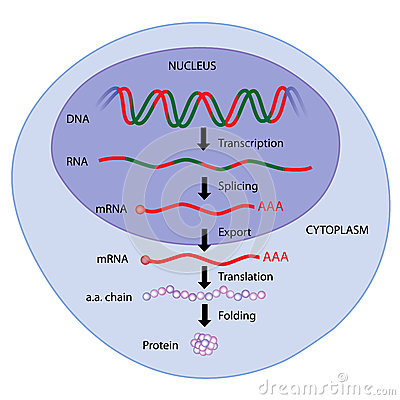
\includegraphics[scale=0.5]{images/dogma_central.jpg}
\caption{Dogma central de la biología molecular}
\label{fig:dogma}
\end{figure}


\subsection{Biología computacional}

Desde los descubrimientos de Watson y Crick, la biología molecular ha crecido de la mano de un sinfín de tecnologías que le han permitido abordar de forma cuantitativa el estudio de fenómenos a escala molecular. Desde el microscopio hasta los modernos secuenciadores, todos los descubrimientos han estado asentados sobre una base tecnológica muy fuerte, de la que han carecido otras áreas de la biología. 

\medskip
Una de las ramas tecnológicas que más ha evolucionado y aportado a la biología molecular en los últimos 30 años ha sido la informática. Esta rama ha  permitido procesar y almacenar de forma ordenada cantidades enormes de datos en tiempos de cómputo razonables. A la aplicación de la informática a la biología y su unión a otras disciplinas como la estadística o las matemáticas, se le denominó biología computacional.
  
\medskip 
La biología computacional, también denominada bioinformática, es una disciplina en la que, a partir de la combinación de modelos, algoritmos y computadores, es posible abordar la resolución de problemas de tipo biológico. Los problemas más característicos afrontados en el pasado mediante la biología computacional han estado relacionados con el alineamiento de secuencias, lo que ha permitido, entre otras cosas, construir árboles filogenéticos que describen como evolucionan y se relacionan las especies cercanas con sus ancestros comunes.

\medskip
En los últimos años, el volumen de datos aportados por la biología molecular ha crecido de forma considerable, lo que ha generado una gran dependencia a nivel informático que ha obligado a la incorporación de procedimientos y herramientas informáticas que permiten automatizar ciertos procesos casi cotidianos.  

\medskip
Entre los logros más importantes de la biología molecular y computacional destaca el Proyecto Genoma Humano \cite{pgh}, encargado de la determinación total de la secuencia de nucleótidos que compone el genoma humano. Esta tarea requirió más de 13 años de trabajo y una inversión superior a 280.000 millones de dólares, aportados mayoritariamente por los gobiernos de Gran Bretaña y Estados Unidos. La descripción de la secuencia del genoma humano y la localización de los genes tuvo una gran relevancia en los ámbitos de la biomedicina y la genética clínica, permitiendo arrojar luz sobre las bases moleculares de algunas enfermedades hereditarias.

\section{Enfermedades de origen genético}

\subsubsection{Enfermedades hereditarias}

Las enfermedades de origen genético son síndromes donde un error en la maquinaria de síntesis de proteínas provoca un comportamiento anómalo de las células y como consecuencia, la aparición de una enfermedad. Típicamente, su origen viene determinado por una mutación o variación estructural nociva en uno o varios genes, provocando un daño en cadena.

\medskip

Cuando la enfermedad está causada por un único gen, decimos que es monogénica o mendeliana (en honor a Gregor Mendel). Ejemplos de enfermedades monogénicas son la fibrosis quística (causada por el gen \textit{CFTR})\cite{fq}, la enfermedad Huntington (causada por el gen HTT)\cite{huntington}, o la Hemofilia de tipo A (causada por el gen F8)\cite{hemofilia}. Por el contrario, cuando la enfermedad está causada por la combinación de varios genes mutados, entonces decimos que es multigénica. Las enfermedades multigénicas son mucho más frecuentes que las monogénicas, y engloban a la mayoría de enfermedades crónicas como la hipertensión, la obesidad, o síndromes complejos como el alzheimer o la esquizofrénia. 

\medskip
Cuando la enfermedad es de carácter familiar, entonces decimos que es hereditaria. En este caso, la mutación o mutaciones nocivas se segregan de padres a hijos. Sin embargo, no todos los individuos portadores acabarán desarrollando la enfermedad, depende del modelo de herencia de la enfermedad. 

\subsubsection{Estructura genómica y modelos de enfermedad}

Los humanos disponemos de un genoma redundante compuesto por 23 pares de cromosomas, lo que significa a efectos prácticos (y a excepción de los cromosomas sexuales) que disponemos de dos copias iguales de cada gen, donde una copia vendrá proporcionada por vía paterna y la otra por vía materna. 

\medskip
*** figura cromosomas en la célula punto de recombinarse

\medskip
Esta duplicidad génica tiene efectos beneficiosos, tanto sobre el individuo como sobre la especie, ya que genera (por combinación) biodiversidad, haciéndonos más resistentes a enfermedades. Sin embargo, también tiene efectos funcionales ya que, cada parental dispone de variaciones estructurales y mutaciones propias que generan pequeñas diferencias entre las dos copias génicas que recibe cada descendiente. 

\medskip
Cuando una mutación está presente sólo en una copia, entonces decimos que se presenta en heterocigosis, sin embargo cuando la mutación es compartida por ambas copias, es decir, ambos parentales disponían de ella, entonces decimos que está presente en homocigosis. 

\medskip
Cuando una enfermedad hereditaria muestra una herencia de tipo recesivo, significa que será necesario disponer de una mutación nociva en ambas copias del gen para acabar desarrollando la enfermedad, lo que generalmente estará asociado a una pérdida de función del gen, ya que ninguna de sus proteínas acabará siendo funcional. Sin embargo, cuando la herencia de la enfermedad es de tipo dominante, entonces significa que, o bien, la copia intacta no es capaz de compensar la ausencia de la copia mutada, o bien la proteína mutada dispondrá de una nueva función que resultará nociva para la célula.  

\medskip
Comprender como funcionan los distintos modelos de enfermedad resulta absolutamente fundamental, ya que nos permite entender las bases moleculares de las enfermedades y por consiguiente, avanzar en su prevención y cura. Además, nos permite ser mucho más eficientes a la hora de buscar genes que puedan estar implicados en una enfermedad con un origen genético total o parcialmente desconocido. El problema se complica cuando las variaciones genómicas no son responsables en su totalidad del inicio de la enfermedad. En este caso, las condiciones ambientales (como los hábitos alimenticios o el clima) explican un porcentaje significativo del riesgo a desarrollar la enfermedad. Existen enfermedades como el cáncer de pulmón, donde los hábitos (como ser fumador) juegan un papel decisivo en su riesgo y proliferación, y otras enfermedades, principalmente monogénicas, donde presentar ciertas variaciones estructurales asegura una penetrancia casi total, con independencia de los hábitos del individuo.

\medskip
Dentro del estudio de enfermedades hereditarias, es de especial interés el estudio de enfermedades raras. Las enfermedades raras, o también conocidas como huérfanas, son aquellas que tienen una baja incidencia en la población (inferior a 5 de cada 10.000 individuos) y por su condición de baja prevalencia, son sometidas a menores inversiones por parte de capital público y privado. Existen más de 7000 enfermedades raras descritas por la OMS y se estima que afectan al 7\% de la población mundial (sólo en España afectan a más de 3 millones de personas). Este tipo de síndromes se benefician claramente de las estrategías de secuenciación de genoma completo, ya que de otra forma, serían necesarios costosos estudios previos que focalizaran el origen de la enfermedad sobre un grupo reducido de genes candidatos.

\medskip
Panorama mundial /penetrancia/ ***

\subsubsection{Repositorios de polimorfismos y mutaciones}

\medskip
1000 genomas: mutaciones en población sana ***

\section{Secuenciación de ADN}

\subsection{La secuenciación del genoma}

La secuenciación del ADN nos permite conocer el orden específico de los nucleótidos en el genoma de un individuo, lo que posteriormente facilita la identificación y localización de los genes. Comparando la secuencia obtenida con una secuencia de referencia es posible determinar aquellas diferencias o variaciones estructurales que presenta un individuo y que podrían ser susceptibles de haber causado o causar una enfermedad en el futuro. La construcción de un genoma de referencia con el que comparar ya supone de por sí un reto tecnológico importante que ha sido llevado a cabo en la última década. Además, el genoma de referencia constituye una plantilla sana con la que comparar y definir la normalidad no es algo sencillo. Esta importante tarea recae sobre un consorcio internacional \cite{GRC} encargado de construir y almacenar la versión oficial del genoma humano, actualizándolo de forma periódica.

\medskip
La secuenciación de genomas o porciones de ADN ha sido llevada a cabo por medio de diferentes procedimientos a lo largo de los últimos 50 años. Los métodos implementados han permitido determinar con fiabilidad la secuencia de nucleótidos correspondiente a un fragmento de material genético. Todos los métodos han mostrado tasas de error cuantificables y parámetros críticos como su complejidad, facilidad de ejecución, velocidad de secuenciación o coste económico, los cuales han sido claves para su evolución y adopción por parte de los investigadores. 

\medskip
Uno de los principales handicaps producidos por el desarrollo de tecnología heterogénea es que cada método de secuenciación ha venido acompañado de su propia base científica y de numerosas herramientas y métodos estadísticos de análisis específicos, lo que ha requerido un reaprendizaje de las herramientas de trabajo por parte de los investigadores. Este hecho ha tenido especial incidencia en los últimos años ya que cada tecnología ha dado lugar a una batería de herramientas informáticas de análisis y de algoritmos encargados de resolver problemas específicos de cada tecnología. 

\medskip
A continuación, se enumeran tres de las metodologías de secuenciación más empleados en la biología molecular. Cabe destacar que a pesar de mostrar una cronología clara, todos los métodos son actualmente vigentes y es habitual verlos coexistir en proyectos genómicos, donde cada tecnología es usada en su ámbito adecuado. 


\subsection{Secuenciación por \emph{Sanger}}

El método de secuenciación más empleado en las últimas décadas ha sido el denominado método \emph{Sanger} \cite{sanger}, en honor a su creador Frederick Sanger. Sanger, el cual es una de las 4 personas que han recibido un premio Nobel dos veces en su vida, fue capaz de demostrar que las proteínas tienen una estructura específica y que esta es fundamental para su función. Para ello, consiguió en 1955 determinar la secuencia de aminoácidos de la insulina y desarrolló un método con el que obtuvo un perfil específico de su estructura \cite{sanger_estructura}. Este trabajo le permitió obtener su primer nobel de química en 1958. Años más tarde (en 1975) desarrolla formalmente su método de secuenciación \cite{Sanger1977}, el cual, a partir de dideoxinucleótidos, un gel de agarosa y la aplicación de electroforesis fue capaz de obtener un patrón de bandas a partir del cual es posible deducir la secuencia subyacente de nucleótidos. 

\medskip
Con este método, Sanger secuenció al bacteriófago A4, que se convirtió en el primer organismo cuyo genoma fue secuenciado de forma completa. Los trabajos de Sanger fueron fundamentales en la consecución del \emph{Proyecto Genoma Humano} y en otros ambiciosos proyectos de secuenciación posteriores, gracias a lo cual fue galardonado con su segundo nobel de química en 1980. 

\subsection{Chips de ADN}

A pesar de los importantes avances obtenidos mediante la secuenciación por Sanger, ha sido necesario evolucionar a formas más rápidas y automáticas de secuenciación que dejaran atrás algunas limitaciones técnicas como la secuenciación de largas cadenas de ADN. Con una perspectiva sistémica, se ha evolucionado hacia métodos de secuenciación que son capaces de obtener información simultanea de miles de genes. 

\medskip
Una de las tecnologías más populares surgidas en la última década han sido los chips de ADN, los cuales, gracias su buena relación coste/prestaciones se extendieron rápidamente a la gran mayoría de estudios biomédicos con una componente genómica importante.

\medskip
Un chip de ADN se compone de una matriz de sondas (o pocillos), donde cada elemento es capaz de medir información concreta acerca de un gen. Los chips más empleados han sido los de expresión génica. Estos, recogen en cada pocillo una porción de la secuencia complementaria de cada gen, a partir de la cual son capaces de obtener una medida proporcional a la abundancia de ARN mensajeros y por tanto de la expresión de los genes. 

*** figura microarrays

\medskip
Otros chips ampliamente extendidos, han sido los chips de genotipado. En este caso, el chip se encarga de testar la presencia de una cantidad enorme de polimorfismo en la secuencia de los genes, que actuan sobre marcadores genómicos asociados a enfermedades.

\medskip
Si bien, los chips de ADN no han constituido una tecnología capaz de obtener la secuencia precisa de nucleótidos de cada gen, sí han servido de forma eficiente y barata para la determinación algunas características esenciales relacionadas con la dinámicas de los genes.

\subsection{Ultrasecuenciadores o técnicas de secuenciación masiva}

Los avances de la última década han permitido el desarrollo de técnicas de secuenciación másiva a un coste muy bajo. Se trata de tecnologías que permiten procesar y secuenciar simultáneamente millones de fragmentos de ADN. Son las llamadas tecnologías de ultrasecuenciación o secuenciación másiva y son capaces de secuenciar un genoma completo en aproximadamente una semana, con un coste inferior a 20.000 dolares, algo que hace 15 años habría sido difícil de imaginar. Lógicamente, estas técnicas han revolucionado la genómica computacional, dirigiendo los estudios hacia una perspectiva más genómica que génica.

\medskip
A pesar de sus numerosas prestaciones, los técnicas de secuenciación másiva también muestran algunas limitaciones importantes. La más destacada reside en la longitud máxima que los aparatos son capaces de secuenciar. Actualmente, los secuenciadores son capaces de obtener fragmentos de entre 50 y 500 nucleótidos, lo cual, comparado con técnicas clásicas como la secuenciación por Sanger, resulta muy pobre. Además, los fragmentos de ADN secuenciados tienen que volver a ser reposicionados sobre el ADN para poder reconstruir el genoma completo de la muestra y los secuenciadores no aportan ningún tipo de información a este respecto. Por esta razón, es necesario realizar un paso de computado adicional denominado \emph{mapeo} donde cada fragmento secuenciado se compara con un genoma de referencia. Algunos parámetros, como la longitud del fragmento, serán claves para la fiabilidad del mapeo, ya que, a menor tamaño, más probable será encontrar la misma secuencia de nucleótidos en varios puntos del genoma. 

\medskip
Otra limitación importante reside en la tasa de error obtenida durante la determinación de la secuencia de nucleótidos, la cual es superior al resto de técnicas de secuenciación. Por esta razón, es habitual realizar un análisis estadístico a partir de datos de ultrasecuenciación, complementados con una fase de validación posterior realizada por el método \emph{Sanger}.

\medskip
A pesar de todo, los ultrasecuenciadores constituyen una tecnología más que prometedora que aporta un enfoque genómico muy eficiente en el estudio de aquellas enfermedades donde los genes causantes de la enfermedad son desconocidos


\section{Identificación de genes candidatos}


\subsection{Regiones de interés}

Los genes constituyen únicamente el 5\% del genoma, el resto, antaño considerado como ADN basura [***], tiene una función todavía desconocida, que en algunas ocasiones estará relacionada con aspectos más estructurales que funcionales en la molécula de ADN. A su vez, los genes tienen en su interior cierto grado de estructura. Poseen porciones que serán codificadas directamente a proteínas, llamadas exones o regiones codificantes, pero también poseen otras regiones dedicadas al control de su expresión, e incluso otras regiones, denominadas intrones, implicadas en la formación de las diferentes isoformas del gen.

\medskip
\begin{figure}
\centering
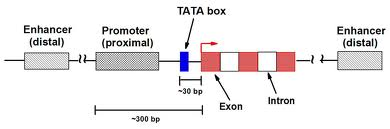
\includegraphics[scale=1]{images/estructura_gen.jpeg} 
\caption{Estructura de un gen}
\end{figure}

\medskip
Debido a la estructura y funcionamiento del genoma, se considera mucho más probable encontrar una mutación causante de enfermedad dentro de una zona codificante, ya que esta produciría un cambio directo sobre las proteínas generadas y por consiguiente, un comportamiento anómalo. Esta circunstancia produce que en la práctica no se realice una secuenciación orientada a genoma completo, por el contrario, se recurre a kits especiales de secuenciación que cubren únicamente las regiones codificantes de los genes. Esta reducción en el área de búsqueda, que puede tener implicaciones serias en casos donde la mutación nociva no afecta a una zona codificante sino a una zona reguladora, permite en la práctica trabajar sólo con el un 2\% del total del genoma, lo cual aporta grandes beneficios para toda la fase de procesamiento, almacenamiento y análisis que ocurre después de la secuenciación, consiguiendo un aprovechamiento máximo de los recursos económicos disponibles dentro de un proyecto de investigación. 

\subsection{Estudio caso/control}

El protocolo de selección de genes candidatos se realiza a partir de un estudio caso/control. En este caso, se trata de identificar a aquellos genes mutados que podrían tener una relación directa con la enfermedad. Como es habitual, el grupo de casos está formado por una serie de individuos que comparten el mismo síndrome, en este caso, de origen genético. 

\medskip
El grupo de casos se acompaña de un grupo de individuos control que nos permite filtrar todas aquellas mutaciones potencialmente nocivas que por estar presentes en población sana no deberían estar relacionadas con el síndrome. 

\medskip
Una vez realizada la secuenciación y el resto de pasos computacionales necesarios, se obtienen todas las mutaciones propias de cada individuo del estudio, descartando a aquellas que no muestren un efecto nocivo probado. Las mutaciones seleccionadas, serán sometidas, generalmente, a un test estadístico de proporciones (como el test exacto de Fisher) que identificará a aquellos candidatos de mayor prevalencia en casos frente a controles. Cabe destacar que este proceso puede realizarse a nivel mutacional, donde todos los individuos enfermos compartirán exactamente el mismo cambio nocivo, o a nivel génico, donde lo importante es identificar al gen mutado, por encima de las variaciones estructurales propias de cada individuo enfermo.

\medskip
Debido a limitaciones relacionadas con el tamaño muestral y otro tipo de sesgos surgidos durante todo el proceso, el gen, o genes causantes serán seleccionados junto a un grupo de genes aleatorios que cumplirán los mismos requisitos y que por tanto no podrán ser filtrados ni separados de estos. Será tarea de estrategias posteriores encontrar argumentos biológicos o técnicos que permitan reducir el número de candidatos y priorizar convenientemente a los que quedan, ya que, los mecanismos de validación posteriores son complejos e incorporan de forma habitual costosos trabajos de laboratorio. El tamaño muestral y otros parámetros de calidad relacionados con la secuenciación condicionarán claramente la talla del conjunto de genes candidatos, aunque otros aspectos relacionados con la fase computacional también podrían tener gran influencia.


\subsection{Reducción y priorización de genes candidatos}

La identificación de los genes implicados en el origen de una enfermedad hereditaria constituye una tarea ardua, con unos requerimientos temporales y económicos considerables, en la que es habitual enfrentarse al estudio detallado de cientos de genes candidatos. En este contexto, es necesario contar con protocolos de priorización (manuales o automáticos) que permitan reducir la lista de candidatos iniciales o priorizar convenientemente a los seleccionados en función de criterios biológicos.

\medskip
El proceso de priorización establece un ranking de genes que estima la relevancia de cada candidato sobre los procesos biológicos que se presuponen clave en la enfermedad de estudio, siendo los mejor priorizados aquellos que serán empleados en los análisis posteriores. Los criterios empleados hasta la fecha para determinar la implicación de un gen sobre una enfermedad son muy amplios. En general, se comienza haciendo uso de la estructura de los individuos del estudio caso/control, para posteriormente, recopilar propiedades inherentes a los genes que describen su relevancia global, y en consecuencia, permite modular las probabilidades a priori de cada candidato propuesto. 

\medskip
La selección de genes candidatos comienza generalmente por la delimitación de aquellas regiones del genoma que podrían contener al gen o genes causantes. Esta tarea se ha llevado a cabo por medio de estudios que relacionan zonas cromosómicas con rangos fenotípicos, o en casos familiares, a partir de la intersección entre las zonas mutadas de uno o varios individuos enfermos con sus parentales también afectados.

\medskip
Desgraciadamente, las técnicas de posicionamiento no consiguen centrar convenientemente el problema sobre una reducida lista de regiones que todavía contenga al gen de la enfermedad. Además, muestran algunas limitaciones claras, especialmente en síndromes de origen regulatorio, donde es difícil delimitar las regiones cromosómicas afectadas, y no tienen en cuenta el plegamiento tridimensional de los cromosomas que provoca que dos genes cercanos en el espacio, aparezcan alejados al tratar la secuencia de ADN como un fragmento lineal. A pesar de todo, constituyen un buen punto de inicio, y permiten filtrar algunas regiones candidatas que sólo aportarían ruido al análisis.

\medskip
El uso de información funcional acerca de los genes permite establecer de forma eficiente criterios cuantitativos y cualitativos de \emph{culpabilidad} sobre los candidatos. Las bases de datos con información biológica describen cómo los genes intervienen en rutas metabólicas y de señalización \cite{kegg}, qué funciones biológicas desempeñan en la célula y en qué compartimentos\cite{go}, qué mutaciones han sido descritas previamente \cite{dbsnp} y en qué enfermedades han sido implicadas \cite{hgmd}, así como otro tipo de anotaciones biológicas que pueden tener gran relevancia a la hora de obtener un perfil específico de cada gen. 

\medskip
La información cubre generalmente las siguientes áreas:

\bigskip
\begin{itemize}{}{}
\item \emph{Redes de interacción proteína-proteína:}\\ Interacciones físicas entre las proteínas generadas por los genes.
\item \emph{Anotaciones funcionales:}\\Funciones biológicas, compartimentos celulares y otros roles asignados a las proteínas.
\item \emph{Rutas metabólicas y de señalización:}\\Diagrama de las diferentes rutas biológicas en las células y su implicación en algunas enfermedades.
\item \emph{Asociación a enfermedades:}\\Asociaciones descritas en la literatura de tipo gen/enfermedad o mutación/enfermedad.
\item \emph{Expresión:}\\Expresión de los genes por tejido o momento del desarrollo.
\item \emph{Conservación:}\\Grado de conservación de la secuencia de nucleótidos entre diferentes especies cercanas.
\item \emph{Redes de regulación:}\\Relaciones entre genes reguladores y regulados.
\item \emph{Minería de textos:}\\Frecuencia de aparición de un gen en publicaciones científicas, junto a otros términos relativos a enfermedades, procesos biológicos u otras entidades de interés.
\end{itemize}

\bigskip
El concepto de priorización computacional, tal y como hoy lo conocemos, fue introducido por primera vez en 2002 por Perez-Iratxeta\cite{perez-iratxeta}. A partir de ese momento, multitud de métodos y algoritmos, en su mayoría de uso libre, han sido desarrollados para llevar a cabo tal tarea \cite{review1,review2,review3}. Los métodos propuestos consiguen clasificar y priorizar de forma automática grandes cantidades de genes, lo que los hace muy adecuados en estudios de genoma completo, especialmente en el estudio de aquellas enfermedades genéticas de origen desconocido y cuando el número de candidatos es grande.

\medskip
En general, la inmensa mayoría de métodos propuestos tratan de recuperar la información disponible sobre aquellos genes que ya se han descrito en la enfermedad, con el fin de establecer un criterio de priorización sobre los nuevos candidatos. El mecanismo habitual consiste en obtener un vector de características sobre los genes de referencia, que posteriormente será empleado para medir el grado de similitud entre cada candidato y los genes conocidos, siendo el gen más similar el de mejor priorización. Esta metodología reposa sobre la idea básica de que aquellos genes de enfermedad que todavía no han sido descritos, deberían tener características funcionales, similares a los genes existentes. 


\medskip
%Es conocido que no todas las mutaciones en genes van a producir los mismos efectos. Hay mutaciones que ni siquiera provocan un cambio de aminoácido en la secuencia proteíca, y %otras que directamente impiden la síntesis de la proteina. 
%Mutaciones sinónimas/no sinónimas, No todas las mutaciones causan los mismos síntomas o la misma intensidad de la enfermedad ***




\subsection{Validación del conjunto final de genes candidatos}

***modelos animales


***grupo de test


\section{Metodologías de priorización en ausencia de genes conocidos}


\medskip
La metodología habitual presenta algunas limitaciones. En primer lugar, es necesario disponer de una lista de genes previamente descritos para la enfermedad de estudio, algo que no siempre ocurre. En estos casos, aquellos procesos biológicos relevantes podrían aportar una lista de genes cercanos con los que establecer una referencia secundaria. Por otro lado, la mayor parte de enfermedades mendelianas, disponen de muy pocos genes descritos, lo que a nivel estadístico, supone un problema importante durante la fase de construcción del perfil.


